\documentclass[11pt,a4paper]{article}

\usepackage[T1]{fontenc}
\usepackage[utf8]{inputenc}
\usepackage{lmodern}
\usepackage[margin=24mm]{geometry}
\usepackage{microtype}
\usepackage{booktabs}
\usepackage{amsmath}
\usepackage{longtable}
\usepackage{tabularx}
\usepackage{array}
\usepackage{enumitem}
\usepackage{xcolor}
\usepackage{xurl}
\usepackage{hyperref}
\usepackage{listings}
\usepackage{tikz}
\usetikzlibrary{arrows.meta,positioning,shapes.geometric,fit}

\definecolor{TessarisNavy}{HTML}{071D31}
\definecolor{TessarisBlue}{HTML}{1878D1}
\definecolor{TessarisMint}{HTML}{16806B}
\definecolor{TessarisPale}{HTML}{F2F8FC}
\definecolor{TessarisLine}{HTML}{D7E4ED}
\definecolor{TessarisAmber}{HTML}{A66A00}
\hypersetup{colorlinks=true,linkcolor=TessarisBlue,urlcolor=TessarisBlue,citecolor=TessarisMint}
\setlist[itemize]{leftmargin=*,itemsep=3pt,topsep=4pt}
\setlist[enumerate]{leftmargin=*,itemsep=3pt,topsep=4pt}
\renewcommand{\arraystretch}{1.22}
\newcolumntype{Y}{>{\raggedright\arraybackslash}X}
\newcommand{\code}[1]{\texttt{#1}}
\newcommand{\pathcode}[1]{\path{#1}}
\newcommand{\status}[1]{\textbf{\textcolor{TessarisMint}{#1}}}

\lstdefinestyle{tessaris}{
  basicstyle=\ttfamily\small,
  backgroundcolor=\color{TessarisPale},
  frame=single,
  rulecolor=\color{TessarisLine},
  breaklines=true,
  columns=fullflexible,
  showstringspaces=false
}

\title{\textbf{Tessaris Agent-to-Agent Network and Agent Commerce Protocol}\\[4pt]
\large Technical Architecture, Features, Security Boundaries and Production Status}
\author{Tessaris AI}
\date{27 September 2026}

\begin{document}
\maketitle

\begin{abstract}
This document specifies the implemented Tessaris Agent-to-Agent (A2A) and
Agent Commerce foundation.  The system allows a customer-side agent to express
an outcome, search multiple Tessaris businesses, open guarded commercial
requests, receive comparable offers, and present a time-sensitive shortlist to
the customer.  A business-side agent receives the corresponding work inside
the Tessaris desktop application.  The current implementation provides signed
agent identity, replay protection, idempotent request creation, capability
discovery, durable task state, fee-transparent offers and exact human approval.
It deliberately does not create a booking, take payment, change a calendar or
send an external message when an offer is accepted.  The protocol is functional
on the local Tessaris service; public Internet relay and production market
deployment remain separate release gates.
\end{abstract}

\tableofcontents
\newpage

\section{Purpose and Product Model}

Traditional search returns links and leaves the user to identify suppliers,
compare incomplete information and repeat the same enquiry.  Tessaris instead
implements an intent-to-transaction market:

\begin{enumerate}
  \item the customer describes the required outcome, location, timing, budget
        and authority boundary;
  \item the customer agent searches the available Tessaris business network;
  \item requests are fanned out only to businesses that publish a matching
        capability and service area;
  \item each business agent may inspect the request and prepare a live offer;
  \item Tessaris returns a comparable shortlist containing price, availability,
        terms and the evidence that actually exists;
  \item the customer chooses an exact offer; and
  \item booking, payment, dispatch, fulfilment and final settlement proceed as
        separately authorised stages.
\end{enumerate}

The customer agent is not designed to accept the first price received.  Its
role is to test the available market, identify genuine job fit and clearly
separate live offers from indicative catalogue values.  When reviews or
completed-job evidence do not exist, the interface reports that absence rather
than fabricating reputation.

\subsection{Example outcome}

A request such as ``I need an emergency plumber in Essex today'' may produce:

\begin{itemize}
  \item two businesses that explicitly publish emergency plumbing in Essex;
  \item one live offer valid for thirty minutes and one indicative hourly rate;
  \item availability and alternative time windows;
  \item disclosed terms and the Tessaris facilitation fee;
  \item ``no reviews yet'' where no review evidence exists; and
  \item ``completed jobs not verified'' until completion evidence is available.
\end{itemize}

\section{Implementation Status}

\begin{table}[ht]
\centering
\begin{tabularx}{\textwidth}{>{\bfseries}p{42mm}Y>{\raggedright\arraybackslash}p{32mm}}
\toprule
Component & Current capability & State \\
\midrule
Business agent channel & Automatically created on first use for each Tessaris workspace & \status{Implemented} \\
Capability publication & Services, descriptions, areas, pricing mode, indicative price, availability and terms & \status{Implemented} \\
Agent Card and AgentMap & Machine-readable discovery for a selected business & \status{Implemented} \\
External agent identity & Ed25519 challenge verification and per-request signatures & \status{Implemented} \\
Market search & Multi-business discovery, fan-out and evidence-labelled comparison & \status{Implemented} \\
Commercial tasks & Durable requests, messages, offers, state and artifacts & \status{Implemented} \\
Exact offer approval & Hash-bound human acceptance with no implied payment or booking & \status{Implemented} \\
Desktop interface & Live channel status, capabilities and durable inbound task summary & \status{Implemented} \\
Customer market page & Browser-agent identity, signed search and comparison interface & \status{Implemented locally} \\
Public Internet relay & Publicly reachable ingress, routing and operational service & \textbf{Not deployed} \\
Booking and payment & Provider connectors, reservation and settlement & \textbf{Separate future stage} \\
\bottomrule
\end{tabularx}
\caption{Agent Commerce implementation boundary.}
\end{table}

The accurate product statement is:

\begin{quote}
\textbf{The Tessaris Agent Commerce protocol is functional on the local
Tessaris runtime.  External public availability, booking and settlement are not
yet production-enabled.}
\end{quote}

\section{System Topology}

\begin{figure}[ht]
\centering
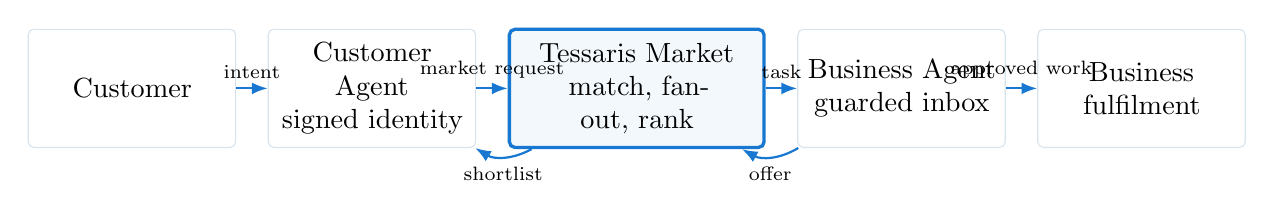
\begin{tikzpicture}[
  node distance=4mm and 4mm,
  box/.style={draw=TessarisLine,fill=white,rounded corners=2pt,minimum height=15mm,text width=24mm,align=center},
  core/.style={box,draw=TessarisBlue,very thick,fill=TessarisPale},
  flow/.style={-{Latex[length=2mm]},thick,draw=TessarisBlue}
]
\node[box] (user) {Customer};
\node[box,right=of user] (ca) {Customer Agent\\signed identity};
\node[core,right=of ca,text width=30mm] (market) {Tessaris Market\\match, fan-out, rank};
\node[box,right=of market] (ba) {Business Agent\\guarded inbox};
\node[box,right=of ba] (business) {Business\\fulfilment};
\draw[flow] (user)--node[above,font=\scriptsize]{intent}(ca);
\draw[flow] (ca)--node[above,font=\scriptsize]{market request}(market);
\draw[flow] (market)--node[above,font=\scriptsize]{task}(ba);
\draw[flow] (ba)--node[above,font=\scriptsize]{approved work}(business);
\draw[flow,bend left=30] (ba) to node[below,font=\scriptsize]{offer} (market);
\draw[flow,bend left=30] (market) to node[below,font=\scriptsize]{shortlist} (ca);
\end{tikzpicture}
\caption{The market provides comparison and authority while direct business
tasks provide the underlying transport.}
\end{figure}

\subsection{Roles}

\begin{description}[style=nextline,leftmargin=18mm]
  \item[Customer] Defines the outcome and remains the final authority unless a
  separately verified delegation policy is introduced.
  \item[Customer agent] Holds a verified network identity, searches the market,
  compares candidates and carries the customer's bounded negotiation context.
  \item[Tessaris market] Matches capabilities, creates per-business tasks,
  assembles evidence-labelled candidates and applies deterministic ranking.
  \item[Business agent] Receives requests within the correct workspace and may
  prepare a commercial offer using authorised business information.
  \item[Business operator] Reviews or approves business-side decisions and later
  provides the real service, product or fulfilment.
\end{description}

\section{Business Channel and Capability Publication}

Opening the Agent Network inside Communications calls the protected status
route.  If the workspace has no commerce profile, Tessaris creates a safe
default profile with:

\begin{itemize}
  \item an enabled local inbound channel;
  \item no published capabilities;
  \item no automatic booking;
  \item no automatic payment; and
  \item human approval as the default transaction policy.
\end{itemize}

The channel is therefore available without falsely advertising services.  A
business must publish at least one real capability before it can appear in a
market result.  Each capability supports the following fields:

\begin{longtable}{>{\ttfamily}p{38mm}p{98mm}}
\toprule
Field & Purpose \\
\midrule
\endhead
service\_id & Stable machine identifier derived from or supplied with the service. \\
name & Customer-readable product or service name. \\
description & Specific work the business can genuinely perform. \\
locations & Permitted service areas; an empty list means that location has not restricted discovery. \\
pricing\_mode & Quote-required, hourly, fixed-price, discovery-first or another declared mode. \\
base\_price\_minor & Indicative catalogue value stored as integer minor currency units. \\
currency & Three-letter currency code, currently defaulting to GBP. \\
availability & Human-readable availability rule or confirmation requirement. \\
terms\_summary & Short terms or commercial boundary made visible during comparison. \\
\bottomrule
\end{longtable}

Capability publication is performed through a signed desktop session.  It is
not an unauthenticated public write operation.

\section{Discovery Artifacts}

\subsection{Agent Card}

The Agent Card exposes the business agent name, endpoint, version, transport,
input and output modes, skills and required signature scheme.  It uses an
A2A-aligned structure with protocol version \code{1.0.0}.  The Tessaris-specific
commerce vocabulary is declared as the extension
\code{urn:tessaris:agent-commerce:v1}.

The card also states operational facts that prevent capability inflation:

\begin{itemize}
  \item discovery is not merely a mock response;
  \item facilitation fees are disclosed;
  \item booking is disabled at this stage; and
  \item payment is disabled at this stage.
\end{itemize}

\subsection{AgentMap}

AgentMap is the Tessaris business-discovery extension.  It binds:

\begin{itemize}
  \item the business identifier and display name;
  \item the corresponding Agent Card URL;
  \item accepted protocol names;
  \item the published capability catalogue;
  \item commercial task, status, message and offer-approval routes;
  \item the authority boundary; and
  \item hashes of the Agent Card and AgentMap content.
\end{itemize}

AgentMap remains a Tessaris extension rather than a claim that every field is
part of the upstream A2A standard.

\section{External Agent Identity and Request Authentication}

\subsection{Registration challenge}

An external agent supplies an agent identifier, display name and raw 32-byte
Ed25519 public key.  Tessaris returns a random, five-minute challenge.  The
agent signs the canonical JSON challenge payload.  Successful verification
activates the public key for that identifier.

An existing active agent identifier cannot be silently rebound to a different
public key.  This prevents a newly generated key from taking over tasks that
belong to the original identifier.

\subsection{Signed request format}

Every protected external request signs the following exact byte sequence:

\begin{lstlisting}[style=tessaris]
METHOD\n
PATH\n
TIMESTAMP\n
NONCE\n
SHA256_BODY
\end{lstlisting}

The request carries:

\begin{itemize}
  \item \code{X-A2A-Agent-ID};
  \item \code{X-A2A-Timestamp};
  \item \code{X-A2A-Nonce}; and
  \item \code{X-A2A-Signature}.
\end{itemize}

Tessaris rejects an unverified identity, invalid signature, malformed
timestamp, request older than five minutes, invalid nonce and any nonce that
has already been used.  Accepted nonces are stored durably so replay protection
survives a process restart.

\subsection{Abuse controls}

The external boundary includes durable fixed-window rate limits.  Challenge
issuance is limited by client address, challenge verification is separately
limited, and signed requests are limited by agent identity.  Both public A2A
requests and protected desktop A2A controls have a 64 KiB pre-routing request
body ceiling.  Oversized bodies are rejected before Pydantic or business logic
parses them.

\section{Market Search and Multi-Business Fan-out}

A market search contains:

\begin{itemize}
  \item requested service or product;
  \item outcome description;
  \item location;
  \item requested time window;
  \item maximum budget in integer minor units;
  \item currency; and
  \item negotiation authority metadata.
\end{itemize}

The current deterministic matching stage tokenises the requested outcome and
published service metadata.  A candidate is eligible when the service is an
exact identifier match or shares meaningful terms, and its published locations
do not conflict with the requested location.  A separate commercial task is
created for every eligible business, up to the bounded fan-out limit.

Each search has its own market identifier and task set.  A repeated request
with the same customer-agent identity and idempotency key returns the original
search instead of opening duplicate business work.

\subsection{Candidate evidence model}

Each candidate includes:

\begin{itemize}
  \item matched business and capability;
  \item task identifier;
  \item availability;
  \item price amount, currency and evidence state;
  \item facilitation fee when a live offer exists;
  \item terms;
  \item review state and review count;
  \item completed-job evidence state;
  \item offer hash when available; and
  \item the next permitted action.
\end{itemize}

Price evidence is one of:

\begin{description}[style=nextline,leftmargin=18mm]
  \item[\code{LIVE\_OFFER}] The business agent prepared the exact offer; the
  value may be accepted while it remains open and unexpired.
  \item[\code{INDICATIVE\_CATALOGUE}] A published starting or catalogue price;
  it is not represented as a confirmed quotation.
  \item[\code{QUOTE\_PENDING}] No price has yet been supplied.
\end{description}

Reviews use \code{NOT\_AVAILABLE} until real review evidence exists.
Completed-job counts use \code{NOT\_VERIFIED} until a verified completion
source is connected.  Zero and unknown are not treated as the same fact.

\subsection{Ranking}

The current ranking order is deterministic:

\begin{enumerate}
  \item specific job/capability match;
  \item requested service area;
  \item live offer ahead of indicative price;
  \item available evidence quality; and
  \item total customer-facing price.
\end{enumerate}

Alphabetical business name is used only as a stable final tie-breaker.  Future
reputation ranking must be evidence-backed, explainable and resistant to paid
placement being misrepresented as relevance.

\section{Commercial Tasks and Offers}

\subsection{Task state}

Each business request is durably stored with an A2A-style task identifier,
context identifier, business, customer agent, status, intent, authority,
messages, offers, artifacts and timestamps.  A request with a valid service
enters \code{working}; a request that lacks capability selection enters
\code{input-required}.

Task access is isolated in both directions:

\begin{itemize}
  \item a customer agent can read or update only its own task; and
  \item a business desktop can read or prepare offers only for its own
        workspace.
\end{itemize}

\subsection{Fee-transparent offer calculation}

Amounts use integer minor currency units.  For service price $S$, facilitation
fee rate $r$ in basis points and tax $T$, Tessaris calculates:

\[
F = \operatorname{round}_{\mathrm{half\ up}}\left(\frac{S r}{10000}\right),
\qquad
C = S + F + T,
\]

where $F$ is the Tessaris facilitation fee and $C$ is the total customer-facing
amount.  The service price, basis-point rate, fee, tax and total are all carried
inside the offer.  The offer also records scope, terms, availability, expiry,
creator digest and an immutable SHA-256 offer hash.

\subsection{Exact approval}

Acceptance is bound to the exact offer hash.  The human confirmation phrase is:

\begin{lstlisting}[style=tessaris]
APPROVE <offer_hash>
\end{lstlisting}

An expired, missing, already closed or mismatched offer cannot be accepted.
Successful acceptance records an acceptance hash and completes the negotiation
task.  It explicitly records:

\begin{itemize}
  \item \code{payment\_created = false}; and
  \item \code{booking\_created = false}.
\end{itemize}

This prevents an agreement to commercial terms from being mistaken for money
movement, calendar reservation or dispatch.

\section{Dynamic and Surge Pricing Boundary}

The protocol can later carry dynamic prices for taxis, emergency trades,
limited inventory and other time-sensitive markets.  The current market record
states:

\begin{itemize}
  \item dynamic pricing is not yet enabled; and
  \item undisclosed surge pricing is not allowed.
\end{itemize}

A future dynamic-pricing release should require a declared pricing basis,
normal reference price, multiplier or adjustment, reason, expiry, maximum cap
and customer-facing disclosure.  Ranking must use the final all-in amount, not
an artificially low pre-surge figure.  The user must see that the price is
dynamic before approval.

\section{Desktop Communications Interface}

The Communications \texorpdfstring{$\rightarrow$}{->} Agent Network page now
contains a live protocol panel.  It displays:

\begin{itemize}
  \item local versus publicly relayed channel state;
  \item protocol version;
  \item verified external agent count;
  \item open request and waiting-offer counts;
  \item Agent Card and AgentMap URLs;
  \item published business capabilities;
  \item capability publication controls; and
  \item a summary of durable inbound agent work.
\end{itemize}

The page distinguishes the implemented network from the older Phase 14 and
Phase 18 preview panels.  Legacy preview panels remain available for historical
scenario inspection, but they are not the source of truth for the live channel.

Desktop mutations use the existing HMAC-protected AION Flow desktop session.
The Electron signer allowlist now includes only the
\code{/api/aion/business/a2a/} prefix in addition to the previously approved
protected surfaces.  The renderer never receives the desktop session secret.

\section{Customer Market Interface}

The local customer doorway is served at \code{/market}.  It provides a simple
natural-language search experience while retaining protocol-level identity:

\begin{enumerate}
  \item the browser generates a temporary Ed25519 keypair;
  \item it completes the A2A identity challenge;
  \item it signs the exact market-search request;
  \item Tessaris returns the multi-business candidate set;
  \item the page clearly labels live, indicative and pending prices; and
  \item an enabled acceptance control appears only for an exact live offer.
\end{enumerate}

The page states that search is not a purchase and that offer acceptance does
not create a booking or take payment.  It is intentionally useful as a visible
website while remaining compatible with the longer-term goal that most traffic
will arrive through personal agents and machine APIs.

\section{HTTP API Surface}

\begin{longtable}{>{\ttfamily}p{18mm}>{\ttfamily}p{72mm}p{52mm}}
\toprule
Method & Route & Function \\
\midrule
\endhead
GET & \pathcode{/.well-known/agent-card.json} & Discover a business Agent Card. \\
GET & \pathcode{/agentmap.json} & Retrieve the Tessaris AgentMap. \\
GET & \pathcode{/.well-known/agentmap.json} & Retrieve AgentMap from the well-known path. \\
GET & \pathcode{/market} & Open the customer market interface. \\
POST & \pathcode{/api/a2a/v1/agents/challenge} & Create an agent identity challenge. \\
POST & \pathcode{/api/a2a/v1/agents/verify} & Verify the challenge signature and activate the agent. \\
POST & \pathcode{/api/a2a/v1/market/search} & Search and fan out across eligible businesses. \\
GET & \pathcode{/api/a2a/v1/market/{market_id}} & Refresh the evolving candidate set. \\
POST & \pathcode{/api/a2a/v1/tasks} & Open a direct guarded business task. \\
GET & \pathcode{/api/a2a/v1/tasks/{task_id}} & Read authorised task status. \\
POST & \pathcode{/api/a2a/v1/tasks/{task_id}/messages} & Continue negotiation or supply requested facts. \\
POST & \pathcode{/api/a2a/v1/tasks/{task_id}/approve} & Accept the exact live offer. \\
POST & \pathcode{/api/aion/business/a2a/status} & Read or initialise the protected workspace channel. \\
POST & \pathcode{/api/aion/business/a2a/profile} & Publish protected business capabilities. \\
POST & \pathcode{/api/aion/business/a2a/inbox} & Read the workspace's durable task inbox. \\
POST & \pathcode{/api/aion/business/a2a/tasks/{task_id}/offers} & Prepare a business-side offer. \\
\bottomrule
\end{longtable}

\section{Persistence and Auditability}

The default runtime root is
\code{AIONBusinessPaths.ROOT/a2a\_commerce}.  State is written atomically to
owner-controlled JSON files and material lifecycle events are appended to a
JSON Lines journal.  The runtime includes:

\begin{itemize}
  \item business profiles;
  \item verified external agents;
  \item expiring identity challenges;
  \item accepted request nonces;
  \item direct-task idempotency mappings;
  \item market-search idempotency mappings;
  \item task documents;
  \item market documents;
  \item rate-limit state; and
  \item append-only event summaries.
\end{itemize}

Event records contain identifiers, timestamps and payload hashes rather than a
full duplicate of customer message content.  Private market content remains in
the corresponding task and market records.  A production service should move
these stores to an encrypted, backed-up database with explicit retention,
legal-hold and deletion policies.

\section{Security and Privacy Properties}

\subsection{Implemented properties}

\begin{itemize}
  \item Ed25519 proof of possession for external agent identities.
  \item Exact method, path, timestamp, nonce and body-hash binding.
  \item Five-minute request freshness window.
  \item Durable nonce replay rejection.
  \item Agent identifier key-replacement protection.
  \item Durable idempotency for direct tasks and market searches.
  \item Workspace isolation for business inboxes and offers.
  \item Customer-agent isolation for market and task reads.
  \item Pre-routing payload limits and durable request-rate controls.
  \item Integer monetary arithmetic with explicit rounding.
  \item Hash-bound offer acceptance.
  \item No payment, booking or external messaging side effect in negotiation.
\end{itemize}

\subsection{Information intentionally public through discovery}

A published business name, public service description, service areas,
indicative prices, availability statement and terms summary may appear in an
Agent Card or AgentMap.  Credentials, private customer messages, internal
operator identifiers, desktop session secrets and unrelated business records
must never be included in discovery documents.

\subsection{Claims not yet permitted}

Until the remaining production gates pass, Tessaris must not claim:

\begin{itemize}
  \item that the local channel is globally reachable;
  \item that a negotiated offer is a confirmed booking;
  \item that approval means payment was taken;
  \item that an indicative value is a live quotation;
  \item that a business has reviews or completed jobs when no evidence exists;
  \item that market ranking is independently audited; or
  \item that the implementation is a complete certification of the upstream
        A2A specification.
\end{itemize}

\section{Verification Evidence}

The focused Agent Commerce suite verifies:

\begin{itemize}
  \item Agent Card protocol and capability output;
  \item Ed25519 challenge registration;
  \item signed request verification;
  \item nonce replay rejection;
  \item prevention of agent-identifier key takeover;
  \item idempotent task creation;
  \item forced removal of unapproved full-purchase authority;
  \item transparent twelve-percent fee arithmetic in the reference test;
  \item exact offer-hash approval;
  \item absence of payment and booking side effects;
  \item safe automatic business-channel creation;
  \item workspace isolation;
  \item durable rate limiting;
  \item multi-business market fan-out;
  \item catalogue versus live-offer evidence labels;
  \item missing-review and unverified-job-history labels; and
  \item deterministic candidate reprioritisation after a live offer arrives.
\end{itemize}

The new focused suite reports \textbf{5/5 passing}.  The broader selected A2A
and AgentMap regression run reports \textbf{309/310 passing}.  The remaining
failure is an older source-text lock that scans a broad JavaScript region for
the literal word \code{undefined}; it is not a live protocol or runtime failure.
The installed desktop application was rebuilt and visually verified, and the
local browser market completed a real signed search returning an honest empty
market result when no business capability had been published.

\section{Primary Implementation Files}

\begin{longtable}{p{58mm}p{82mm}}
\toprule
File & Responsibility \\
\midrule
\endhead
\pathcode{backend/modules/aion_business/runtime/a2a_commerce_service.py} & Identity, discovery, persistence, market search, tasks, offers, ranking and approval. \\
\pathcode{backend/modules/aion_business/api/a2a_commerce_api.py} & Public and protected HTTP routes and request validation. \\
\pathcode{backend/modules/aion_business/runtime/request_body_limits.py} & Pre-routing payload limits for the A2A trust boundary. \\
\pathcode{backend/modules/aion_business/static/tessaris-market.html} & Customer market interface and temporary browser agent. \\
\pathcode{desktop/mac/src/app.js} & Communications live-channel, capability and inbound-work interface. \\
\pathcode{desktop/mac/electron/main.js} & Protected desktop request signing allowlist. \\
\pathcode{backend/desktop_app.py} & Desktop runtime router installation. \\
\pathcode{backend/main.py} & Full server router installation. \\
\pathcode{backend/tests/workflow_capsules/test_aion_agent_commerce_protocol.py} & Focused protocol, security and market tests. \\
\bottomrule
\end{longtable}

\section{Production Deployment Gates}

\subsection{Public network ingress}

The installed desktop currently advertises a loopback URL unless
\pathcode{TESSARIS_A2A_PUBLIC_BASE_URL} is configured.  Agents outside the
machine require a public Tessaris relay or a verified business-domain endpoint.
The relay must provide TLS, tenant routing, anti-abuse controls, health checks,
back-pressure, observability and a defined availability target without
transferring business execution authority to the relay.

\subsection{Reputation and completion evidence}

Reviews, completed jobs, cancellations, disputes, response time and quote
reliability require an evidence-backed reputation service.  Early markets must
display empty or unverified states.  The platform must resist review purchase,
self-dealing, duplicated identities and outcome suppression.

\subsection{Booking and dispatch}

Booking requires real calendar or dispatch connectors, resource holds,
conflict detection, expiry and compensation when a provider fails.  A selected
offer must not become a confirmed appointment until the provider returns an
authoritative reservation receipt.

\subsection{Payment and settlement}

Payment requires an approved payment service provider, customer authentication,
refund and dispute flows, fee and tax handling, reconciliation, receipts and
explicit separation between held, captured, released and refunded funds.

\subsection{Operational qualification}

Before unrestricted production release, Tessaris should complete independent
security review, cryptographic review, load and abuse testing, multi-device
recovery exercises, a closed customer pilot, incident procedures and final
production authorisation.

\section{Planned Evolution}

The implementation deliberately lays the transport and authority foundation
for broader markets:

\begin{itemize}
  \item trades and emergency call-outs;
  \item taxis and independent drivers;
  \item physical stock and local delivery;
  \item professional appointments;
  \item discovery visits and custom proposals;
  \item metered digital work;
  \item subscriptions and retained services; and
  \item escrow-ready commercial contracts.
\end{itemize}

The next architectural increments are public relay deployment, business
response automation, verified reputation, availability connectors, exact
booking, protected payment and proof-backed fulfilment.  These should remain
separate stages so that commercial intelligence can improve without silently
acquiring financial or operational authority.

\section{Glossary}

\begin{description}[style=nextline,leftmargin=18mm]
  \item[A2A] Agent-to-Agent protocol concepts used for agent discovery and task interaction.
  \item[Agent Card] Machine-readable description of an agent endpoint, skills and security requirements.
  \item[AgentMap] Tessaris extension publishing business capabilities and commercial routes.
  \item[Business agent] The Tessaris agent representing an authorised business workspace.
  \item[Customer agent] A personal or external agent representing a customer's request and bounded authority.
  \item[Live offer] A hash-bound, expiring offer prepared by the relevant business agent.
  \item[Indicative price] Published guidance that is not a confirmed quotation.
  \item[Market search] One customer request fanned out across eligible Tessaris businesses.
  \item[Minor units] Integer currency representation, such as pence rather than decimal pounds.
  \item[Public relay] Future Internet-reachable service connecting external agents to local business channels.
\end{description}

\vfill
\begin{center}
\small\textcolor{TessarisNavy}{Tessaris Agent Commerce Protocol --- local functional foundation; public production qualification remains open.}
\end{center}

\end{document}
